\documentclass[a4paper,11pt]{article}

\usepackage{stile-generale}
\addbibresource{quantitative_analysis.bib}

%------- Metadati -------
\renewcommand{\Uni}{Bocconi University}
\renewcommand{\Dept}{Department of Social and Political Science}
\renewcommand{\Course}{}
\renewcommand{\Instructor}{Prof.\ Garmain\ Gauthier}
\renewcommand{\AuthorName}{Filippo Panfoli}
\renewcommand{\AuthorID}{3158433}
\renewcommand{\AuthorEmailAddr}{filippo.panfoli@studbocconi.it}
\renewcommand{\GitUser}{PanfoliF}
\renewcommand{\GitRepo}{thesis} % se non vuoi repo: lascia vuoto -> {}
\renewcommand{\ORCIDid}{0009-0000-7861-8036}
\renewcommand{\WebsiteURL}{https://github.com/PanfoliF}
\renewcommand{\DocVersion}{v1.1}
\renewcommand{\LastUpdated}{\today}
%\renewcommand{\Keywords}{}
%\renewcommand{\JEL}{}
 %------------------------

\begin{document}
% alias compilepaper='latexmk -xelatex -output-directory="/Users/filippo/Documents/Lab/Formal Models/Paper Formal Models/build" Tex/main.tex'

%------- Title Page -------
% Pagina 1: title page (senza numero visibile)
\CustomTitlePage{Exploring Linguistic Simplification in Parliaments}{\today}
% \setcounter{tocdepth}{1}
% \tableofcontents
\clearpage
\setcounter{tocdepth}{2}
\tableofcontents
\clearpage
%gggg
\pagenumbering{arabic}
\setcounter{page}{1}
% Da qui in poi: numeri visibili e continui (Abstract = pagina 2)
\pagestyle{fancy}
%\justify

%------- Document -------
\part{Introduction}

\textbf{Session 2, February 16: Grand theories of war and peace}

\begin{itemize}
    \item [***] \parencite{buenodemesquitaPrinciplesInternationalPolitics2013}[Chapter 5]
    \item \parencite{levyCAUSESWARCONDITIONS}
    \item \parencite{lakeWhyIsmsAre2011}
    \item \parencite{lakeChallengesLiberalOrder2021}
    \item \parencite{milnerMythEclecticIR2023}
    \item \parencite{OneWorldRival}
\end{itemize}

\newpage

\section{\cite{buenodemesquitaPrinciplesInternationalPolitics2013} Chapter 5}

\begin{itemize}
    \item War is generally inefficient compared to reaching a negotiated settlement.
    \item The risks of war may be exacerbated by uncertainty, making credible commitments, or winner-takes-all situation.
    \item Some important neorealist hypotheses about international peace and stability do not
    flow logically from that theory’s core assumptions. Other important neorealist hypotheses are falsified by the empirical record.
    \item The link between power transition theory’s assumptions and hypotheses is more clear-cut than is true in the case of neorealism.
    \item Some core power transition hypotheses follow from the theory’s logic and are supported by evidence; others either do not follow logically or are not borne out by evidence.
    \item The power transition theory outperforms neorealism when it comes to offering a structural explanation for war, but its weaknesses point to a need to reconsider its approach to domestic politics.
\end{itemize}

Consider that estimates of war-related deaths per year in the past 100 years vary approximately from 1 to 2 million.

\subsection{War and Uncertainty}
The ex ante problems that seem to lead to war can be reduced to three main factors: (1) uncertainty, (2) commitment problems, and (3) indivisibility of issues (Fearon 1995; Slantchev 2003).

\begin{itemize}
    \item [1] Absence of \textbf{credible commitments} between the sides.
    \item [1.1] The inability to \textbf{commit to negotiating} patiently rather than seizing the first-strike advantage
    exacerbates the risk of war (Powell 1999; Slantchev 2003)
    \item [1.2] The idea is that the Israelis give up
    some land in exchange for a guarantee of peace. An alternative formulation reverses the sequence of concessions—the Palestinian Authority disarms its factions that engage in violence against Israel in return for land concessions. Either approach is likely to fail because each induces a fundamental commitment problem.
    \item [] \textbf{Land for peace} suffers from a time inconsistency problem.
    \item [2] Dispute is about an \textbf{indivisible objective} --> No settlement can produce a compromise in this case of indivisibility, and so there is a severe risk of war. If control over all the land currently held by Israel
    is truly its irreducible objective, then the land is viewed as indivisible by Hamas.
    \item [3] This \textbf{uncertainty about the true probability of victory} or defeat might arise out
    of private (secret) information about the morale of their fighting forces, about knowledge of
    outside help, about the quality of their war plans, or a host of other possible factors.
\end{itemize}

\subsection{Realist Theory}
Neorealist theorists believe that the distribution of power in the international system is a
major factor in determining whether international affairs are stable or unstable. Stability
refers to circumstances in which the sovereignty of key states is preserved (Gulick 1955).
Instability refers to changes in the composition of the international system, especially
changes involving the disappearance or emergence of “key” states following large wars. Key
states are those whose assistance might be necessary to counteract a threat from a rival coali-
tion of states.

In addressing war and instability, neorealist theories start with the following
four assumptions:

\begin{enumerate}
    \item International politics is anarchic. $\Rightarrow$ there is no supranational authority that can enforce agreements between states.
    \item States, as rational unitary entities, are the central actors in international politics. $\Rightarrow$ domestic politics does not influence international politics.
    \item States seek to maximize their security above all else and consider other factors only after security is assured. $\Rightarrow$ states are not willing to trade away their security for other benefits. Other possible goals, such as wealth, are pursued only after security has been assured (Waltz 1979, 126).
    \item States seek to increase their power as long as doing so does not place their security at risk. $\Rightarrow$ states accept being weaker than they might otherwise be if the pursuit of greater power would place their security at risk.
\end{enumerate}

Most important neorealist conclusions
\begin{enumerate}
    \item Bipolar systems are more stable than multipolar systems.
    \item States engage in balancing behavior so that power becomes more or less equally divided
    among states over time.
    \item States mimic, or echo, one another’s behavior.
\end{enumerate}

\newpage

\section{How Well Does Neorealism Do in Explaining War and Instability?}

\subsection{Bipolarity and Stability}
The argument that bipolar structures are more stable than multipolar ones is built on the claim that there is more uncertainty in a multipolar system than in a bipolar one.

Bipolarity is thought to alleviate two of the conditions we have discussed that are thought to increase the risk of war: uncertainty and commitment problems.

There are several problems with the argument that because bipolar systems encompass less
uncertainty than multipolar systems they yield greater stability. This argument is not implied logically by the four key assumptions of neorealism.

\begin{enumerate}
    \item First, variation in the response to uncertainty violates the unitary rational actor assumption, which contends that important choices in international politics are driven by structural factors, not by considerations internal to the state.
    \item Second, if different decision makers respond to uncertainty in different ways, then there is no reason to expect any empirical relationship between bipolarity and stability at all.
    \item Third, if leaders differ in how they respond to uncertainty, then the third hypothesis (that states mimic one another) does not hold up.
    \item taking the neorealist assumptions into account, we can show that it is logically true that more distributions of power are stable in a multipolar world than in a bipolar world. 
\end{enumerate}

\subsection{Bipolarity and Stability 2}
Stability in a multipolar world is not limited to the situation of exact power equality. This is in marked contrast to the bipolar world, in which stability can be achieved only through a perfectly equal division of resources between the two blocs.

Thus, it appears that the first neorealist hypothesis, that bipolarity promotes stability and multipolarity promotes instability, is logically flawed given the assumptions of the theory.

Further, it seems that a true balance of power is essential for stability in a bipolar world, but not in a multipolar one, contradicting the second hypothesis. A vast array of power distributions can produce stability. In a multipolar environment, an exact balance of power is irrelevant.

Either the balance of power does not matter in multipolarity or the term is defined to mean any system in which each actor is essential. In the latter case, so many systems qualify as a balance-of-power system that the concept doesn’t have much meaning in our search for answers.

\subsection{History and Neorealist Empirical Claims}

\begin{enumerate}
    \item The international system was multipolar in structure from 1648 until the defeat of Germany in 1945. Thus, between 1648 and 1945 there were many major powers with no one or two predominating. $\Rightarrow$ The bipolar system began in 1945 and lasted until about 1989.
    \item Using Jack Levy’s (1983) classification of great powers since 1492, we can determine whether the longevity of the bipolar system was comparatively long or short. $\Rightarrow$
    \item Another way to evaluate the stability of the international system is to examine the frequency of wars among the most influential states in the world
    \item The UN Security Council (UNSC), then, by institutionalizing a multipolar decision-making structure, has provided a counterweight to bipolarity. This too may be an explanation for the long peace.
    \item The average interval between general wars is thirty-four years; the longest interval is ninety-nine years, much longer than the so-called long peace. It appears, then, that the bipolar, long peace cannot be considered unusually long after all and that bipolarity is not a superior treatment for the disease of major power war than is multipolarity.
\end{enumerate}

\subsection{Historical Record of Essential and Inessential States}

An essential state is any state that can join a losing coalition and, by dint of its membership and the power it can bring to bear, turn that coalition into a blocking coalition or a winning coalition.

Inessential states are states that are unable to turn even one losing alliance into a winning or blocking coalition.

\begin{enumerate}
    \item Essential states never become inessential.
    \item Essential states are never eliminated from the international system.
    \item Inessential states never become essential states.
    \item Inessential states are always eliminated from the international system.
\end{enumerate}

Each of these propositions is historically false.

\subsection{Balance of Power and Neorealism}
Perhaps the most common claim among neorealist theorists is that war occurs only when both sides believe that their chance of winning is greater than 50 percent. This is a partial statement of what has come to be known as the balance-of-power theory. It invokes the idea that war is the product of mutual optimism by rival states, meaning that they overestimate their chances of victory

If the neorealist hypothesis were correct, we should observe no wars initiated by the weaker side. The evidence fails to support the hypothesis.

\newpage
\section{The Power Transition}
Building on the work of Edward Carr (1939, 1945) and Organski (1958) constructed what was perhaps the first challenge to realism that was neither idealistic nor normative.

\begin{itemize}
    \item The international system is not anarchic.
    \item There is only one dominant state at any given time.
    \item Rather than wishing to maximize security or power, nations are interested in maximizing their \textbf{control over the rules and customs that govern international interactions} so that they can define the status quo according to their interests.
\end{itemize}

Bretton Woods Agreement $\Rightarrow$ These agreements still maintain a rule-based and normative influence on the trading practices of their members.

\textbf{Dissatisfaction} $\Rightarrow$ it is the more powerful dissatisfied states that represent the biggest threat to international peace and stability.

\begin{center}
    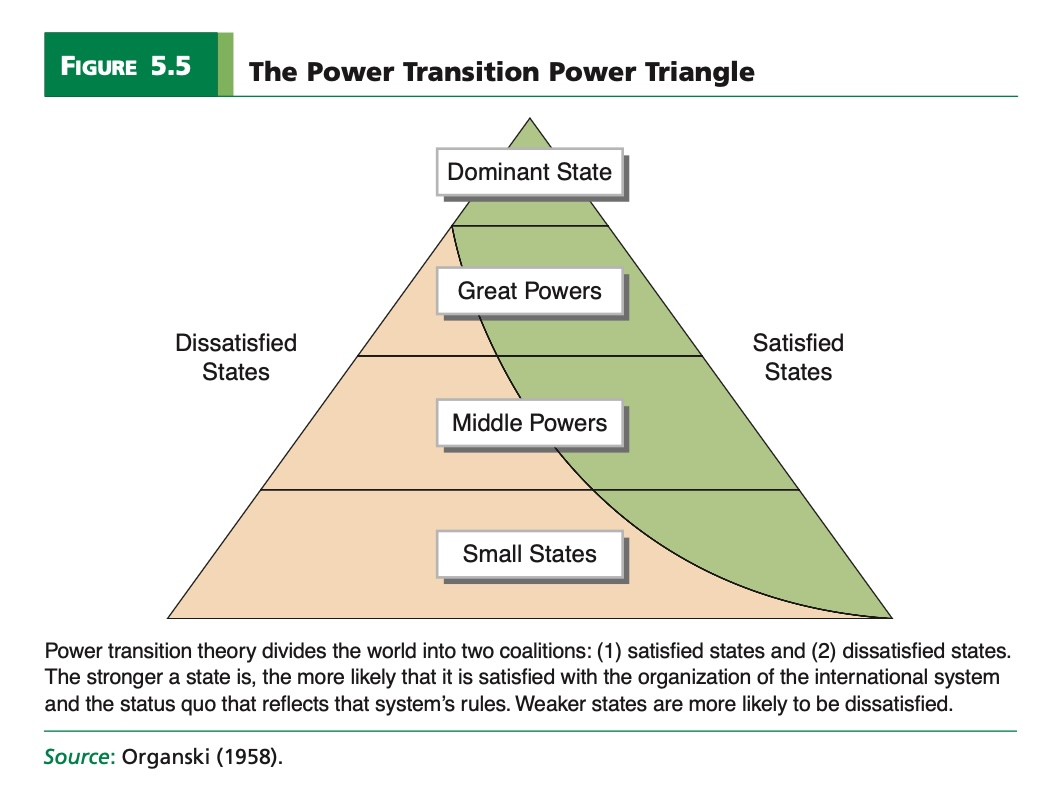
\includegraphics[width=1\textwidth]{images/power_transition_triangle.jpg}
    \captionof{figure}{\label{fig:fig1_power_transition_triangle}%\textit{\parencite[Fig.\(\backsim\)1]{cranmerWhatCanWe2017}}
    }
\end{center}

\subsection{Dissatisfaction, the Status Quo, and War}
Conflict arises when a dissatisfied state grows strong enough to challenge the authority of the hegemon. Because such a challenge concerns the very way in which international affairs are conducted, the ensuing conflict is fierce and costly.

This time period during which the challenger roughly comes to equal and then surpass the dominant state in power is known as the power transition. It is the time when the threat of a major war is hypothesized to be at its peak.
\textbf{Contrary to the balance-of-power perspective}, power transition and hegemonic stability theorists believe that major wars are most likely to occur when the power of the opposed states is about equal.

\textbf{According to these theorists, a balance of power promotes war.} They maintain that system-transforming wars—that is, wars that lead to a new power hierarchy and to new rules and norms—will occur only when the power of a challenger and the dominant state are about equal and the power of the challenger is increasing faster than that of the dominant state. These claims have been extended and shown to have \textbf{empirical strength} at the regional as well as the global level, so that regional hegemons apparently face the same pressures and the same sources of war as their global counterparts.

Threatening balance of power emerges as a result of differing rates of internal growth between a dominant state and a challenger state. These theories still give little attention to domestic politics per se, but they do recognize that internal factors shape rates of growth.

Power transition theory leads to the hypothesis that system-transforming, high-cost wars are especially likely when a dissatisfied challenger state achieves approximate power parity with the dominant, status quo-defending state.

Kim and Morrow have shown that the distribution of power at which the rivals will fight depends on their willingness to take the risks of waiting. The longer the challenger waits to attack, the higher is its probability of victory. This is true because the challenger’s power is growing faster than the dominant state’s power. Thus, the longer the challenger puts off a war, the greater will be the odds in its favor. However, the longer it waits, the longer it must endure the rules of international intercourse with which it is dissatisfied.

Kim and Morrow have shown that the interval during which the challenger is willing to fight expands as the expected costs of the war increase, as the challenger’s dissatisfaction with the status quo increases, as the challenger’s relative growth rate declines, and as the challenger becomes more risk acceptant.

How long the challenger and the dominant states will wait before fighting depends on their respective responses to risk, their relative rates of growth, the expected costs of the war, and their respective degrees of satisfaction with the status quo.

Differences in growth rates turn out not to be crucial empirically.

Power transitions per se cannot explain especially costly wars.

\begin{center}
    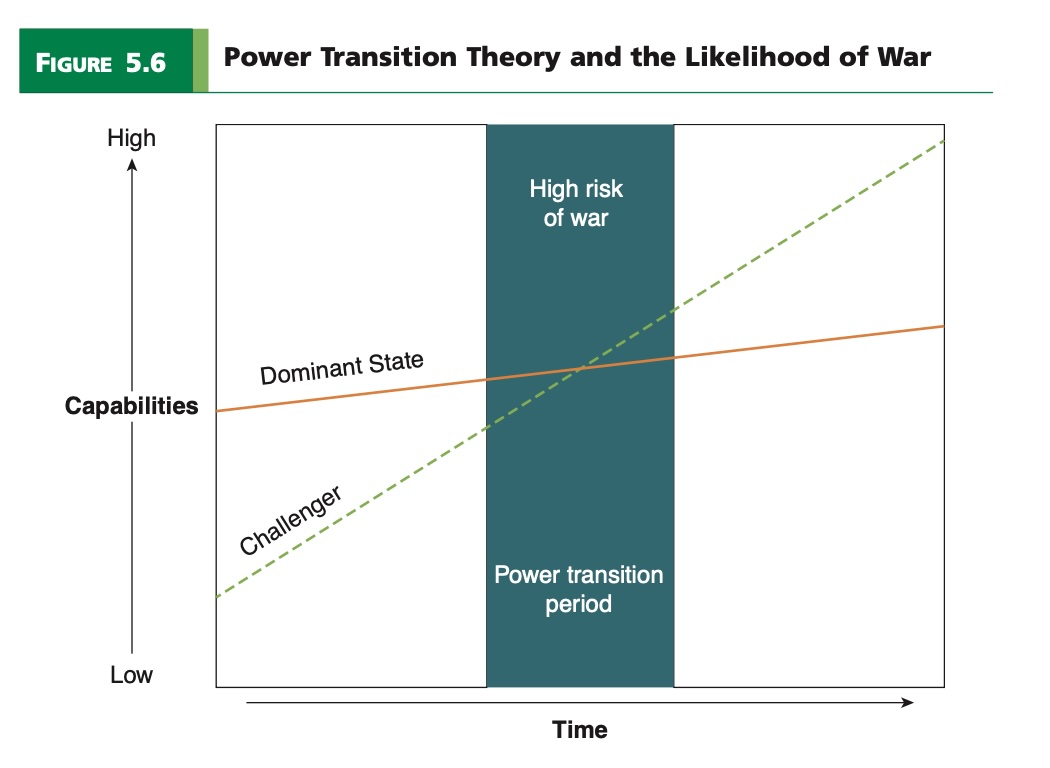
\includegraphics[width=1\textwidth]{images/power_transition_pattern.jpg}
    \captionof{figure}{\label{fig:fig1_power_transition_pattern}%\textit{\parencite[Fig.\(\backsim\)1]{cranmerWhatCanWe2017}}
    }
\end{center}

\newpage

\section{\cite{levyCAUSESWARCONDITIONS}}
This makes it hard to argue that human nature and related factors are causes of war. The point is that these factors are constants and cannot explain the variations in war and peace over time and space (Waltz 1959, Cashman 1993).

Why does war occur at some times rather than other times, between some states rather than other states, under some political leaders rather than others, in some historical and cultural contexts rather than others, and so on? This differs from still a third question: How do we explain the origins of a particular war? Most international relations scholars (and particularly those in North America) focus primarily on the second question, explaining variations in war and peace. They leave the question of why war occurs at all to philosophers and biologists and leave the question of why a particular war occurs to historians.

Although \textbf{anarchy} may provide one persuasive answer to the question of the permissive causes of war, it is generally treated as a structural constant and consequently it cannot account for variations in war and peace.

\subsection{The Levels-of-Analysis Framework}
Waltz (1959) classified the causes of war in terms of their origins in the individual, the nation-state, and the international system $\Rightarrow$ levels-of-analysis framework as an organizing device for the study of war.

In this sense the systemic level of analysis refers to explanations of patterns and outcomes in the international system; the dyadic level refers to explanations of the strategic interactions between two states; the national level refers to explanations of state foreign policy behavior; the organizational level refers to explanations of the behavior of organizations; and the individual level refers to explanations of the preferences, beliefs, or choices of individuals.

We cannot assume that correlations or causal connections at one level of analysis are necessarily valid at another level. It is conceivable, for example, that concentrations of power may promote peace at the dyadic level but war at the system level.

\subsection{Systemic-Level Theories}
The realist tradition has dominated the study of war since Thucydides and includes Machiavellians, Hobbesians, classical balance of power theorists, Waltzian neorealists, and hegemonic transition theorists. Although different realist theories often generate conflicting predictions, they share a core of common assumptions: the key actors in world politics are sovereign states that act rationally to advance their security, power, and wealth in a conflictual international system that lacks a legitimate governmental authority to regulate conflicts or enforce agreements.

\begin{itemize}
    \item they use Prisoner's Dilemma and stag-hunt models
    \item The core proposition of realist theory is that the distribution of power, throughout the system or within a dyad, is the primary factor shaping international outcomes.
\end{itemize}

We should treat realism as a paradigm rather than as a theory, and focus instead on specific theories that generate more determinant, testable propositions.

\subsubsection{Hegemonic Theory or Power Transition Theory}
Hegemonic theory is a structural theory that incorporates power transition theory and hegemonic stability theory and that \textbf{downplays the importance of anarchy}.

Hegemons commonly arise and use their strength to create a set of political and economic structures and norms of behavior that enhance the stability of the system while advancing their own security. Differential rates of growth, the costs of imperial overextension, and the development of vested domestic interests lead to the rise and fall of hegemons, and the probability of a major war is greatest at the point when the declining leader is being overtaken by the rising challenger.

Power transition theorists disagree somewhat on the precise identity of hegemonic wars and the particular causal dynamics from which they arise.

\subsubsection{Balance of Power Theory}
Balance of power theory is more concerned with explaining national strategies, the formation of blocking coalitions, the avoidance of hegemony, and the stability of the system than the origins of wars, which are underdetermined.

There is a major debate, however, between classical realists, who argue that stability is further supported by the presence of a multipolar distribution of power and a “flexible” alliance system (Morgenthau 1967, Gulick 1955), and neorealists, who argue that bipolarity is more stable than multipolarity (Waltz 1979, Mearsheimer 1990).

\textbf{Balance of power theory and power transition theory appear to be diametrically opposed}; the former argues that hegemony never occurs and that concentrations of power are destabilizing, and the latter argues the opposite.

\subsubsection{Realism and Liberalism}
The relationship between economic interdependence and war is an old question that has attracted new attention in the past few years.

\textbf{Liberal economic theory of war:} Montesquieu [1977 (1748)] stated that “peace is the natural effect of trade,” and liberal economic theorists since Smith [1937 (1776)] and Ricardo [1977 (1817)] have argued that capitalist economic systems and the free exchange of goods in an international market economy are the best guarantors of peace.

\textbf{Realist:} they often argue that the effect of trade on war is small relative to that of military and diplomatic considerations. They also question the liberal assumption that trade is always more efficient than military coercion in expanding markets and investment opportunities and in promoting state wealth.

Whether the incentives for the gains from trade dominate the incentives for coercion or protection based on economic asymmetries, and whether the latter escalate to trade wars and militarized conflicts, are empirical questions that analysts have only recently begun to analyze systematically.

\textbf{Historical and empirical evidence of trade between enemies}

Although liberals and realists disagree on the effects of trade on war, \textbf{they appear to agree that trade and other forms of economic interchange between societies will cease or be drastically reduced once states are at war with each other.} Contrary to both liberal and realist expectations, however, \textbf{there are numerous historical cases of trade between enemies} during wartime, and a preliminary quantitative study suggests that war frequently does little to depress the volume of trade between adversaries (Barbieri \& Levy 1997).

Need to incorporate domestic variables into their hypotheses

\textbf{States often hesitate to terminate trade with the enemy for fear that they will lose that trade to a third party}, who may be a greater economic or military rival.

These omissions have led all but the most committed neorealists to conclude that \textbf{systemic-level theories are theoretically incomplete and empirically inadequate}, in that \textbf{they leave too much of the variation in the outbreak and expansion of war unexplained.}


\subsection{Social-Level Theories}

Although interest in Marxist-Leninist theories has waned, there has been a tremendous growth of research on the relationships between regime type, particularly democratic regimes, and war (analyzed by Ray in this volume). Scholars have also devoted attention to the "diversionary" use of force for domestic political purposes, to the impact of ethnonationalism on international conflict, and to other domestic sources of international conflict.

"rally around the flag" effect (Mueller 1973).

This is the age-old "scapegoat hypothesis" or "diversionary theory of war" (Levy 1989a).

As Bodin argued, "the best way of preserving a state, and guaranteeing it against sedition, rebellion, and civil war is to...find an enemy against whom [the subjects] can make common cause" (quoted in Levy 1989a, p. 259).

research on the scapegoat hypothesis

The absence of significant findings regarding the relationship between internal and external conflict contrasts sharply with evidence of external scapegoating from historical and journalistic accounts and from a growing body of case-study evidence.

Most of these studies have focused on democratic regimes, partly because of the ease of measuring elite support levels but also because of the assumption that the greater political accountability of leaders in democratic states makes them more likely than authoritarian leaders to engage in external scapegoating.

These models help to explain "gambling for resurrection" through risky foreign policies by poor leaders who expect to be removed by their constituents (Downs \& Rocke 1995).

This raises the question of how external actors perceive and respond to diversionary actions.

Marxist-Leninist models of imperialism, like models of scapegoating, implicitly assume that external expansion and the use of force serve the interests of the ruling class or elite but not those of society as a whole.

If the costs of aggressive foreign policies are too high---and we have enough examples of "imperial overstretch" to suggest that they sometimes are---it is not clear how elites maintain their power. As Snyder (1991) argued, groups concentrated enough to benefit from overexpansion are too narrow to control state policy, while those broad enough to control policy are too diffuse to reap benefits from overexpansionist policies.

For Snyder, this rationalist model of logrolling is not sufficient to explain overexpansion or the stability of the ruling coalition.

\subsection{Individual-Level Theories}
decision-making is characterized by “bounded rationality”
\textbf{Assumptions:}
\begin{enumerate}
    \item [(a)] that external and internal structures and social forces are not translated directly into foreign policy choices;
    \item [(b)] that key decision-makers vary in their definitions of state interests, assessments of threats to those interests, and/or beliefs as to the optimum strategies to achieve those interests; and
    \item [(c)] that differences in the content of actors’ belief systems, in the psychological processes through which they acquire information and make judgments and decisions, and in their personalities and emotional states are important intervening variables in explaining observed variation in state behaviors with respect to issues of war and peace.
\end{enumerate}

\textbf{Prospect Theory} one of the most recent attempts to apply a social-psychological model to international relations (Kahneman \& Tversky (1979)).

Prospect theory assumes that people evaluate outcomes in terms of deviations from a reference point or aspiration level rather than in terms of net-asset levels.

This asymmetry of behavior with respect to gains and losses means that the way people frame their reference point in any given choice problem is critical.

\subsection{General Trends}

\begin{itemize}
    \item shift away from the systemic level: dissatisfaction with the failure of structural systemic models to explain enough of the variance in war and peace. This shift has led to rising interest in both dyadic-level behavior and societal-level explanatory variables.
    \item Whatever the relationship between concentrations of military and economic capabilities at the systemic level, there is substantial evidence that at the dyadic level an equality of capabilities is significantly more likely to lead to war.
    \item In the past decade most international relations theorists have moved beyond their earlier preoccupation with explanations at a single level of analysis and debates about which level provides the most powerful explanations. They now give much more attention to interaction effects among variables at different levels in the processes leading to war
\end{itemize}


\section{One World Rival Theories}
\textcite{snyderOneWorldRival2004}

\begin{center}
    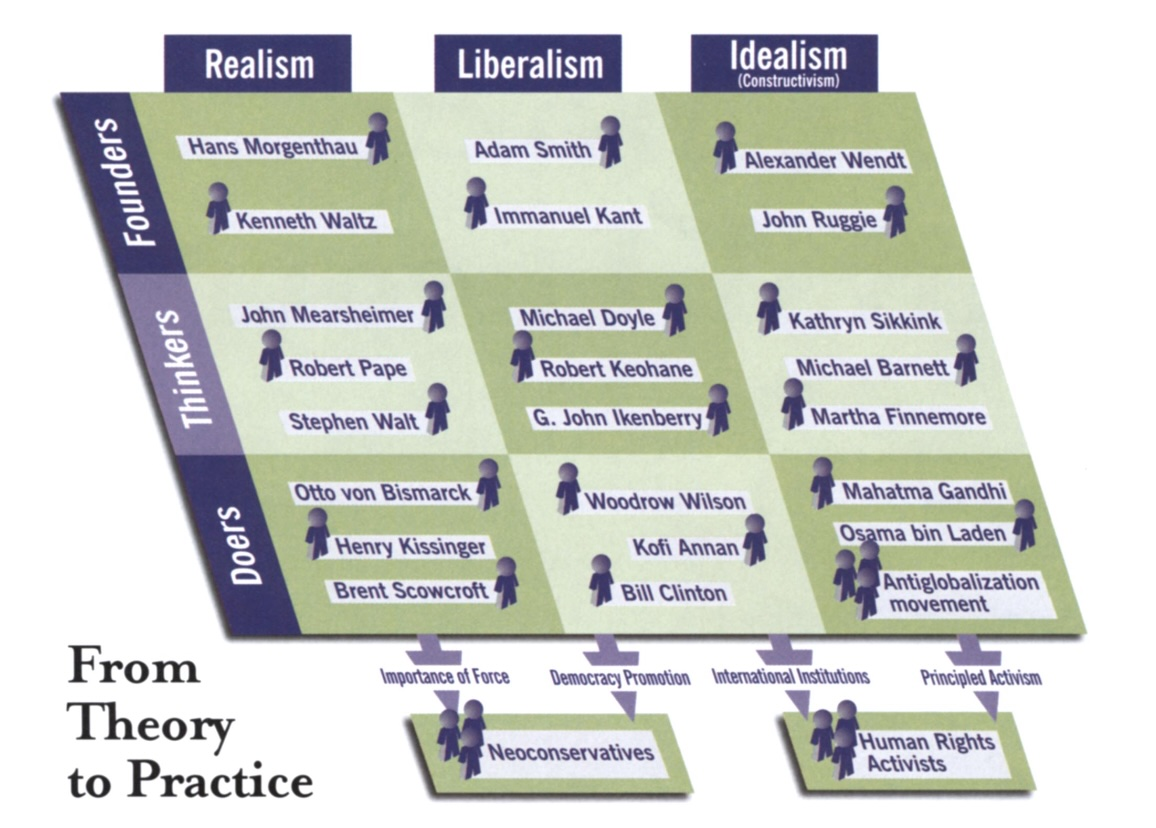
\includegraphics[width=0.7\textwidth]{images/snyder_one_world_rival_theories.jpg}
    \captionof{figure}{\label{fig:fig4_snyder_one_world_rival_theories}%\textit{\parencite[Fig.\(\backsim\)1]{cranmerWhatCanWe2017}}
    }
\end{center}

Realism instills a pragmatic appreciation of the role of power but also warns that states will suffer if they overreach. Liberalism highlights the cooperative potential of mature democracies, especially when working together through effective institutions, but it also notes democracies' tendency to crusade against tyrannies and the propensity of emerging democracies to collapse into violent ethnic turmoil.

Idealism stresses that a consensus on values must underpin any stable political order, yet it also recognizes that forging such a consensus often requires an ideological struggle with the potential for conflict.

It is harder for the normally state-centric realists to explain why the world’s only superpower announced a war against al Qaeda, a nonstate terrorist organization. How can realist theory account for the importance of powerful and violent individuals in a world of states? Realists point out that the

Post-9/11 developments seem to undercut one of realism's core concepts: the balance of power.

When Germany unified in the late 19th century and became Europe's leading military and industrial power, Russia and France (and later, Britain) soon aligned to counter its power. Yet no combination of states or other powers can challenge the United States militarily, and no balancing coalition is imminent.

\subsection{The Divided House of Liberalism}
For its part, the Bush administration highlights democracy promotion while largely turning its back on the international institutions that most liberal theorists champion.

The belief that democracies never fight wars against each other is the closest thing we have to an iron law in social science.

Shortly before September 11, political scientist G. John Ikenberry studied attempts to establish international order by the victors of hegemonic struggles in 1815, 1919, 1945, and 1989. He argued that even the most powerful victor needed to gain the willing cooperation of the vanquished and other weak states by offering a mutually attractive bargain, codified in an international constitutional order.

\begin{center}
    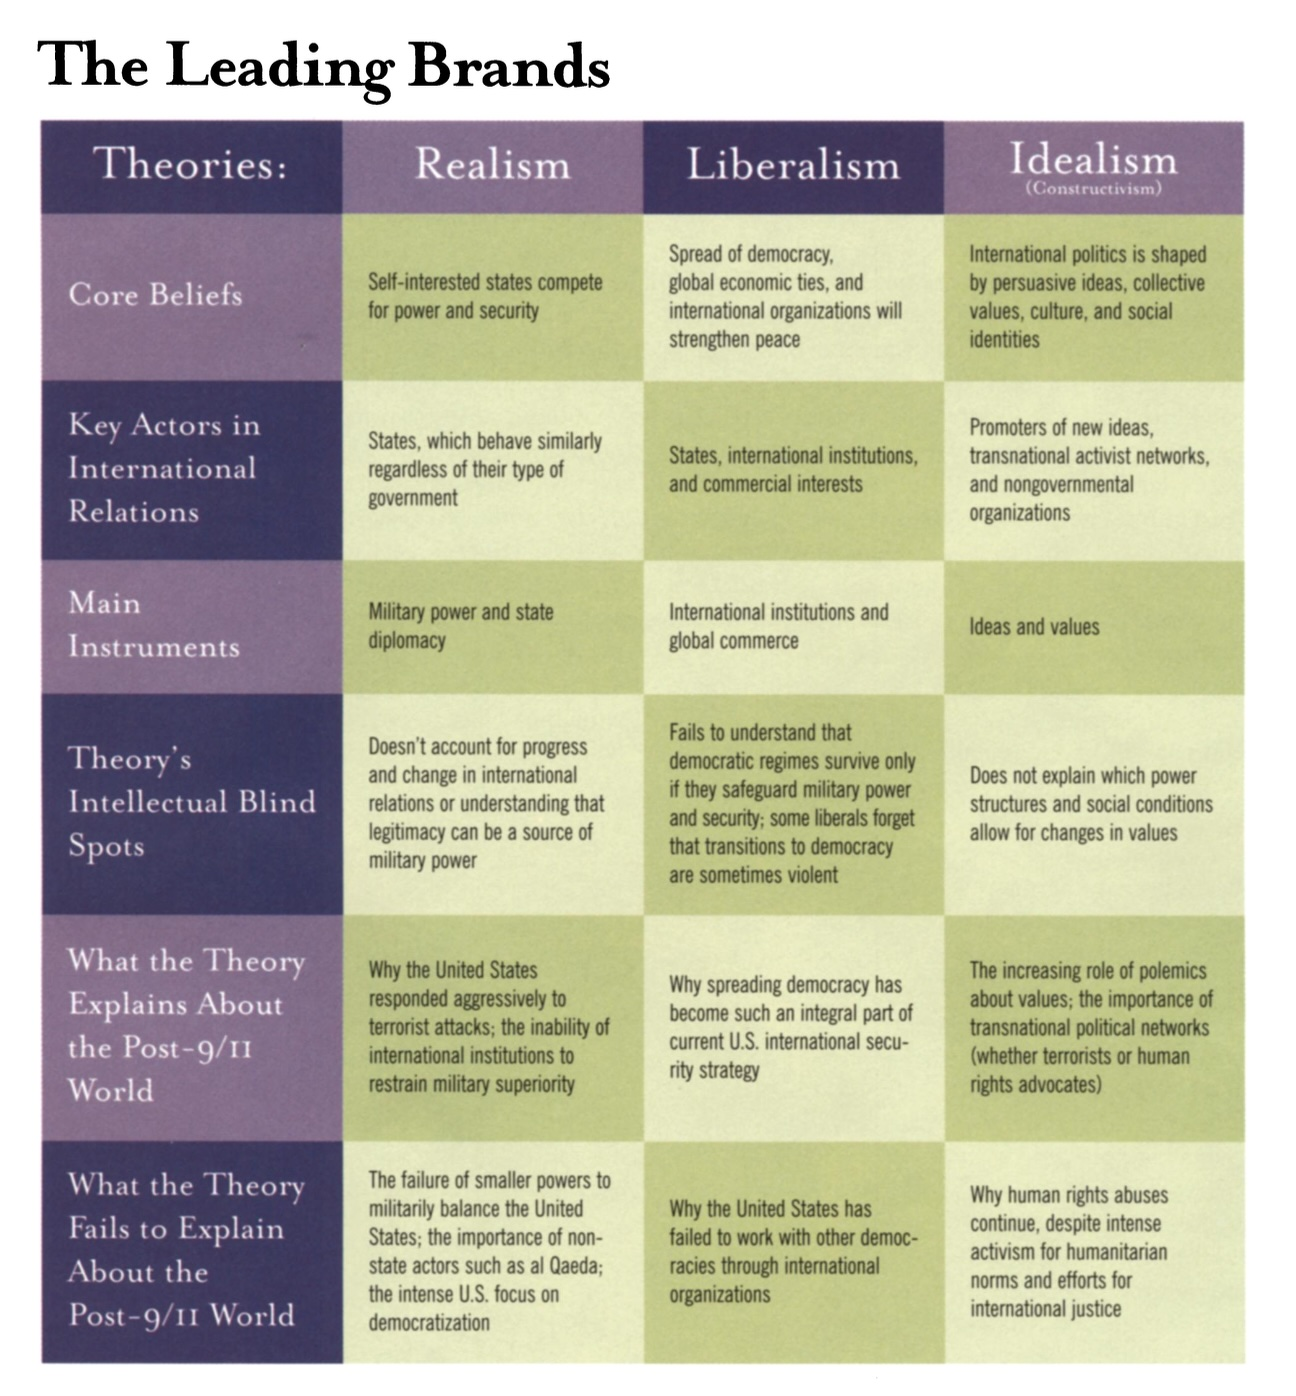
\includegraphics[width=0.7\textwidth]{images/snyder_one_world_rival_theories_the_leading_brands.jpg}
    \captionof{figure}{\label{fig:fig5_snyder_one_world_rival_theories_the_leading_brands}%\textit{\parencite[Fig.\(\backsim\)1]{cranmerWhatCanWe2017}}
    }
\end{center}

\subsection{Idealism}
Idealism: the belief that foreign policy is and should be guided by ethical and legal standards.

\textbf{Constructivism is a new version of idealism:} holds that social reality is created through debate about values, often echoes the themes that human rights and international justice activists sound.

Perhaps most important, Europe’s increasingly legalistic approach to international relations, reflected in the process of forming the European Union out of a collection of sovereign states, provides fertile soil for idealist and constructivist conceptions of international politics.

\textbf{Whereas realists dwell on the balance of power and liberals on the power of international trade and democracy, constructivists believe that debates about ideas are the fundamental building blocks of international life. Individuals and groups become powerful if they can convince others to adopt their ideas.}

Realists failed to predict the end of the Cold War, for example. Even after it happened, they tended to assume that the new system would become multipolar.

Likewise, the liberal theory of democratic peace is stronger on what happens after states become democratic than in predicting the timing of democratic transitions, let alone prescribing how to make transitions happen peacefully.

Constructivists are good at describing changes in norms and ideas, but they are weak on the material and institutional circumstances necessary to support the emergence of consensus about new values and ideas.

With such uncertain guidance from the theoretical realm, it is no wonder that policymakers, activists, and public commentators fall prey to simplistic or wishful thinking about how to effect change.


% !TEX root = ./main.tex
% Summary of David A. Lake (2011), "Why \"isms\" Are Evil"
% This file is intentionally a LaTeX fragment: it does not load a document class
% or packages, so it can be included from your existing main.tex/sty setup.

\section{Why "isms" Are Evil David Lake}
\cite{lakeWhyIsmsAre2011}



\subsection{Central Argument and
Purpose}

Lake's essay is a critique of how international studies is organized
intellectually and professionally. His central claim is not that
theoretical diversity is undesirable, but that scholars have turned
theoretical traditions and epistemological preferences into academic
``sects.'' Instead of using theories as limited tools for understanding
specific problems, researchers often treat broad traditions such as
realism, liberalism, constructivism, Marxism, neoliberal
institutionalism, feminism, or the English School as competing
intellectual religions. Each group tends to defend its own assumptions,
produce research that confirms those assumptions, and debate rival
traditions at the level of first principles. In Lake's view, this
sectarian organization generates less understanding rather than more. It
also distracts scholars from their fundamental social responsibility:
improving knowledge of world politics and, where possible, identifying
ways to promote more humane outcomes.

The problem is especially serious because the discipline does not
possess a single, universal and empirically powerful theory of
international politics. World politics is too complex, and existing
knowledge is too incomplete, for one general framework to explain
everything. Lake therefore urges intellectual humility. Scholars should
accept that most theories are partial and contingent, specify the
conditions under which they apply, and concentrate on mid-level
explanations of concrete phenomena. He favors ``analytic eclecticism'':
researchers should be willing to draw on different assumptions and
theories when different problems require different tools. At the
epistemological level, he makes a parallel argument. The divide between
nomological and narrative forms of explanation is real and enduring, but
neither approach is universally superior. Both can produce valid
knowledge, and the relevant question is which approach is most
illuminating for a particular research problem.

\subsection{Theory: How Research Traditions Become Academic
Sects}

International studies has long been divided into what are often called
paradigms, but Lake prefers the term ``research traditions.'' Each
tradition contains a set of core assumptions concerning the relevant
actors in world politics, their interests, the processes through which
they make decisions, and the nature of political interaction. Different
traditions may focus on individuals, groups, states, or other
collectivities; assume that actors seek wealth, power, security, status,
identity, or justice; and portray international politics as
fundamentally conflictual, cooperative, or socially constructed. These
assumptions are useful because they simplify a complex reality and help
researchers identify puzzles. The difficulty arises when scholars forget
that they are simplifications and begin to treat them as complete
theories or even as truths about the world.

Lake argues that the coexistence of many traditions should be expected.
International politics is an exceptionally complicated social system, so
it is unsurprising that different approaches illuminate different parts
of it. The discipline's weakness lies not in pluralism itself but in the
professional practices that transform pluralism into sectarianism. He
identifies five linked pathologies. Together they encourage scholars to
defend approaches rather than explain phenomena, reward intellectual
extremism, and create self-confirming research communities.

\subsection{The first pathology: reifying research
traditions}

The first pathology is the reification of research traditions. Scholars
routinely organize literature reviews, courses, graduate seminars,
handbooks, and disciplinary histories around familiar ``isms.'' This has
practical advantages because it provides a convenient map of a large
literature, but it also creates artificial boundaries. Complex
scholarship is reduced to a few recognizable schools, subtle differences
within traditions disappear, and authors are classified according to
labels they may not accept themselves. Scholars may see their own work
as eclectic and nuanced while categorizing opponents as ``realists,''
``constructivists,'' or ``liberals.'' As a result, intellectual
identities are partly imposed by others. The discipline collectively
produces the very categories that then appear to be natural and
independent objects.

\subsection{The second pathology: rewarding
extremism}

Once research traditions are reified, the discipline rewards the
clearest and most extreme statements of each tradition. Canonical works
such as Waltz's Theory of International Politics, Keohane's After
Hegemony, or Wendt's Social Theory of International Relations become
shorthand for entire approaches. In the process, qualifications and
subtleties are often lost. These iconic texts gain visibility through
citations and teaching, while younger scholars learn that professional
recognition may come from taking a distinctive sectarian position. New
``isms'' and specialized sections of professional associations can also
become vehicles for status and intellectual entrepreneurship. The result
is a centrifugal process in which extremism generates more extremism,
even if the original authors were more nuanced than later portrayals
suggest.

\subsection{The third pathology: confusing traditions with
theories}

The third pathology is the tendency to mistake a research tradition for
a complete theory. A tradition usually supplies broad assumptions, but
those assumptions are rarely sufficient to generate unique, deductively
valid predictions. Lake uses neorealism as an example. Waltz claimed
that anarchy and the desire for survival imply balancing behavior, yet
the same assumptions can also be compatible with cooperation, collective
security, or bandwagoning unless additional assumptions are introduced.
Similar indeterminacy appears in debates over relative versus absolute
gains in neorealism and neoliberalism. This is why several distinct
theories can coexist inside a single tradition---for example, offensive
realism, defensive realism, and neoclassical realism. They share some
core premises but differ in auxiliary assumptions. Because traditions
are often underspecified, they cannot be meaningfully ``tested'' as
wholes. Yet scholars frequently stage empirical contests between
traditions as if each generated clear predictions, producing debates in
which each side can interpret evidence as confirmation.

\subsection{The fourth pathology: selective empirical
focus}

The fourth pathology is empirical selectivity. Researchers tend to study
the topics, periods, and cases in which their preferred tradition is
most likely to perform well. Realists often focus on great-power
security, liberals on economic policy, institutionalists on
institutions, constructivists on norm change, and English School
scholars on socialization and international society. This pattern need
not result from deliberate bias; it can emerge naturally because
scholars test theories where they initially expect them to work, while
journals and publishers also favor positive findings. Nevertheless, the
cumulative consequence is self-confirmation. Each tradition studies its
strongest domain, finds supportive evidence, and then treats that
evidence as proof of general explanatory power. The research tradition
begins to function like theology: evidence is selected to affirm a prior
commitment rather than used to subject theory to demanding attempts at
falsification.

\subsection{The fifth pathology: the search for intellectual
hegemony}

The fifth pathology is the aspiration of each research tradition to
become the dominant scientific paradigm. Scholars often identify
themselves as realists, constructivists, or institutionalists in ways
that imply their preferred approach is broadly superior to alternatives.
Professional incentives reinforce this competition. If a tradition
becomes dominant, its leading scholars gain status, influence, and
control over disciplinary agendas. Because every group fears losing
ground to its rivals, competition for hegemony resembles an arms race:
even scholars who would prefer cooperation feel pressure to defend and
expand their approach. The collective result is worse for everyone.
Rather than acknowledging the limited scope of existing theories,
research communities expend enormous energy debating assumptions such as
whether actors are rational, whether structure or agency matters more,
or whether power, wealth, norms, or identity should be treated as
fundamental. Without comparable theories applied to the same phenomena,
these ``first-principle'' debates cannot be decisively resolved.

\subsection{Lake's Alternative: Problems, Partial Theories, and a Common
Lexicon}

Lake's preferred alternative is to reorganize scholarship around
substantive problems rather than around intellectual sects. Courses,
conference sections, and research agendas could focus on issues such as
war, climate change, development, inequality, genocide, or political
violence. The guiding question would then be ``What do we know about
this problem?'' rather than ``What are the core assumptions of this
school?'' Such an organization would encourage scholars to compare
explanations on the basis of their contribution to understanding a
phenomenon instead of their loyalty to a tradition.

A central part of this alternative is what Lake calls an ``embrace of
partiality.'' Theories should state their scope and boundary conditions
explicitly and identify what they do not explain. A theory is not
weakened merely because it applies only under certain conditions. On the
contrary, clarity about limits improves scientific evaluation because
scholars can distinguish genuine failures from cases outside a theory's
intended domain. Lake proposes that authors should routinely include a
brief statement of boundary conditions and explanatory limitations. This
would also make it easier to combine knowledge from different theories.
His metaphor is the familiar image of several people touching different
parts of an elephant: each theory may capture one part accurately, while
no single theory describes the entire animal.

Lake explicitly rejects atheoretical research. Theories remain necessary
for explaining patterns and identifying causes. His argument is instead
that scholars should use theories flexibly. A researcher might employ a
rational unitary-state model to study war, a theory of individual norms
to investigate global environmental change, and a sectoral
material-interest model to explain trade policy. Using different
theories for different problems should not be treated as intellectual
inconsistency if each theory is appropriate to the question at hand.

\subsection{Interests, interactions, and institutions as a ``Rosetta
stone''}

Analytic eclecticism creates a possible communication problem: if
scholars abandon fixed traditions, the field could become a ``tower of
Babel'' in which theories are too different to compare. Lake therefore
proposes a common lexicon built around three broad concepts: interests,
interactions, and institutions. Any complete theory of politics must
specify who the relevant actors are, what they want, how they interact,
and the institutional environment in which interaction occurs. Actors
may be individuals, groups, organizations, or states. Interests may
involve power, wealth, identity, status, security, or normative goals.
Interactions may involve zero-sum bargaining, cooperation,
socialization, or the reproduction of inequality. Institutions may range
from weak or epiphenomenal arrangements to dense structures that
constitute actors and enable communication itself.

This lexicon is deliberately neutral among traditions. A rationalist
theory may assume groups pursue material interests, while a
constructivist theory may explain interests as socially constituted. A
realist analysis may treat states as the principal actors, while another
approach disaggregates states into domestic groups. Yet both can still
be translated into the same basic questions about actors, interests,
interactions, and institutions. Components can also be modular:
something treated as given in one theory can be explained in another.
Regime type, for example, may be used as an independent variable in a
theory of war and then become the dependent variable in a separate
theory of democratization. The goal is not theoretical unification, but
clearer comparison, better specification, and cumulative knowledge.

\subsection{Epistemology: The Enduring
Divide}

Lake then turns from theory to epistemology. He identifies a deep divide
between nomological and narrative forms of explanation. This cleavage
has shaped major debates in international relations for decades and, in
his view, is harder to bridge than differences among theoretical
traditions. However, he does not believe that one epistemology will or
should defeat the other. Both have long histories, both respond to
different intellectual intuitions, and both can generate valuable
knowledge. The discipline should therefore accept epistemological
diversity rather than politicize it.

\subsection{The nomological approach}

The nomological approach seeks generalizable explanations based on
covering laws or theoretically specified relationships. It typically
uses the hypothetical-deductive method: researchers derive falsifiable
propositions of the form ``if X, then Y'' and test them using designs
that approximate controlled experiments. True experiments offer the
strongest internal validity, followed by quasi-experiments and then
correlational studies such as regression analysis. Causal claims can
emerge either from a strong design that isolates the effect of X on Y or
from a combination of theory and robust empirical association. Lake
notes that much international-relations research relies on the weaker
correlational form. Science in this tradition is iterative: theory
generates hypotheses, evidence tests them, and theories are revised,
extended, or occasionally rejected.

For Lake, generalizability in nomological research depends primarily on
theory rather than on the particular sample used in a test. If a theory
is explicitly intended to apply to all humans, evidence from a narrower
sample can still be relevant provided the test has strong internal
validity. Conversely, findings from a particular population cannot
validate a theory whose assumptions do not extend to that population.
External validity therefore rests on clearly specified scope and
boundary conditions.

\subsection{The narrative approach}

The narrative protocol organizes explanation differently. It begins with
a descriptive order that links events through time and examines how each
development shapes what follows. It then constructs a configurative
order by adjusting an interpretive framework to the historical facts
through a process of abduction. The objective is to produce a convincing
and plausible account of why events unfolded as they did. Narrative
explanations are often richer and more holistic than nomological models
because they emphasize combinations of causes and historically specific
conjunctures. Their weakness, in Lake's view, is that the criteria for
judging causal adequacy are more subjective. Narratives are evaluated in
terms of verisimilitude and interpretive credibility rather than
experimental internal validity.

Lake stresses that epistemology should not be confused with methodology.
A nomological study can use historical case studies and process tracing,
while a narrative analysis can employ large numbers of observations or
statistical techniques. ``Mixed methods'' can improve research by
testing theories in multiple ways, but mixing methods does not by itself
eliminate the distinction between forms of explanation. Method concerns
the techniques used to gather and analyze evidence; epistemology
concerns what counts as a persuasive explanation.

\subsection{Epistemological Sectarianism and Lake's
Recommendations}

The same pathologies that affect theory also affect epistemology.
Scholars reify the nomological and narrative approaches, reward extreme
positions, apply them selectively to problems where they are likely to
succeed, and then claim universal superiority. These preferences have
become politicized within the profession. Epistemological gatekeepers
can influence hiring, resource allocation, publication, and access to
professional networks, encouraging scholars to cluster with others who
share the same standards of explanation. Lake sees no objective basis
for declaring one epistemology universally superior. Scholars may simply
find one form of explanation more intuitively satisfying than another,
much as some people find beauty in mathematics and others in poetry.

Because neither epistemological tradition is likely to eliminate the
other, Lake proposes three principles for coexistence. First, scholars
should recognize the legitimacy of alternative forms of explanation and
respect colleagues who use them. Treating one's own epistemological
intuition as inherently superior is a form of intellectual hubris.
Second, each approach should be judged on its own terms. Narrative work
should be assessed for completeness, plausibility, competing
interpretations, and possible distortion of historical evidence.
Nomological work should be evaluated for logical deduction, valid
operationalization, and sound research design. Third, scholars should
accept that different approaches are likely to work better for different
questions.

Lake illustrates this final point with substantive examples. Narrative
approaches may be especially effective for slow, historically unique
changes in global norms, such as transformations in attitudes toward
slavery or human rights. Such processes unfold over long periods and are
difficult to analyze while holding the social environment constant. By
contrast, nomological approaches may be especially powerful when
interactions are frequent and institutions are stable enough to generate
repeated observations. Research on war and civil war, or on economic
policymaking within established democratic institutions, can often
benefit from this kind of analysis. The crucial question is therefore
not ``Which epistemology is best?'' but ``Which epistemology provides
the greatest insight for this particular problem?''

\subsection{Conclusion}

Lake concludes by returning to the social purpose of scholarship.
Academic privilege is justified by the expectation that scholars will
expand understanding. International studies fails in this responsibility
when it devotes too much energy to theological wars among theoretical
and epistemological camps. Progress comes from asking important
questions about phenomena that remain poorly understood, choosing
theories and methods appropriate to those questions, and evaluating
evidence honestly. At the present stage of the discipline, no
theoretical or epistemological approach merits hegemony. Diversity is
necessary, but diversity should not take the form of isolated
communities that speak mainly to themselves.

The essay's title is therefore deliberately provocative. ``Isms'' are
``evil'' not because realism, liberalism, constructivism, feminism, or
other traditions are useless, but because scholars too often transform
useful intellectual tools into identities and sects. Research traditions
become harmful when they are treated as complete theories, insulated by
selective evidence, and mobilized in struggles for disciplinary
dominance. Lake's alternative is a more modest and problem-centered
social science: partial theories with explicit limits, analytic
eclecticism across traditions, a shared vocabulary of interests,
interactions, and institutions, and mutual respect between nomological
and narrative forms of explanation. The ultimate measure of success
should be whether scholarship improves our understanding of world
politics and contributes, where possible, to social progress.


\section{Challenges to the Liberal Order: Summary}
\begin{center}
\textit{David A. Lake, Lisa L. Martin, and Thomas Risse (2021)}
\end{center}

\subsection{Introduction and Central Argument}

The Liberal International Order (LIO) is under pressure from several directions at once. The authors emphasize that the postwar order has survived serious crises before, so its collapse should not be assumed.

The LIO has structured relations among the capitalist, democratic, and industrialized states since the late 1940s and has had wider global effects. It is associated with unprecedented cooperation among North America, Western Europe, and Japan, the emergence of a pluralistic security community, expansion of trade and capital mobility, high economic growth, the diffusion of democracy, and the development of an international human-rights regime.

\subsection{Order}

An order consists of patterned or structured relations. The LIO is clearly rule-governed and sustained by coordinated action by both state and nonstate actors.

\subsection{International and the Westphalian Order}

The "international" component of the LIO has to be understood in relation to the Westphalian order. In the authors' usage, Westphalia is not literally a system created in 1648 but a later order centered on sovereign nation-states, sovereign equality, recognition by other states, and noninterference in domestic affairs. The LIO and the Westphalian order partly overlap and have coevolved since 1945. They share principles such as sovereign equality, peaceful settlement of disputes, self-determination, and nonintervention. At the same time, the LIO goes beyond Westphalia through principles such as human rights and forms of legitimate collective intrusion into domestic affairs.

\begin{center}
    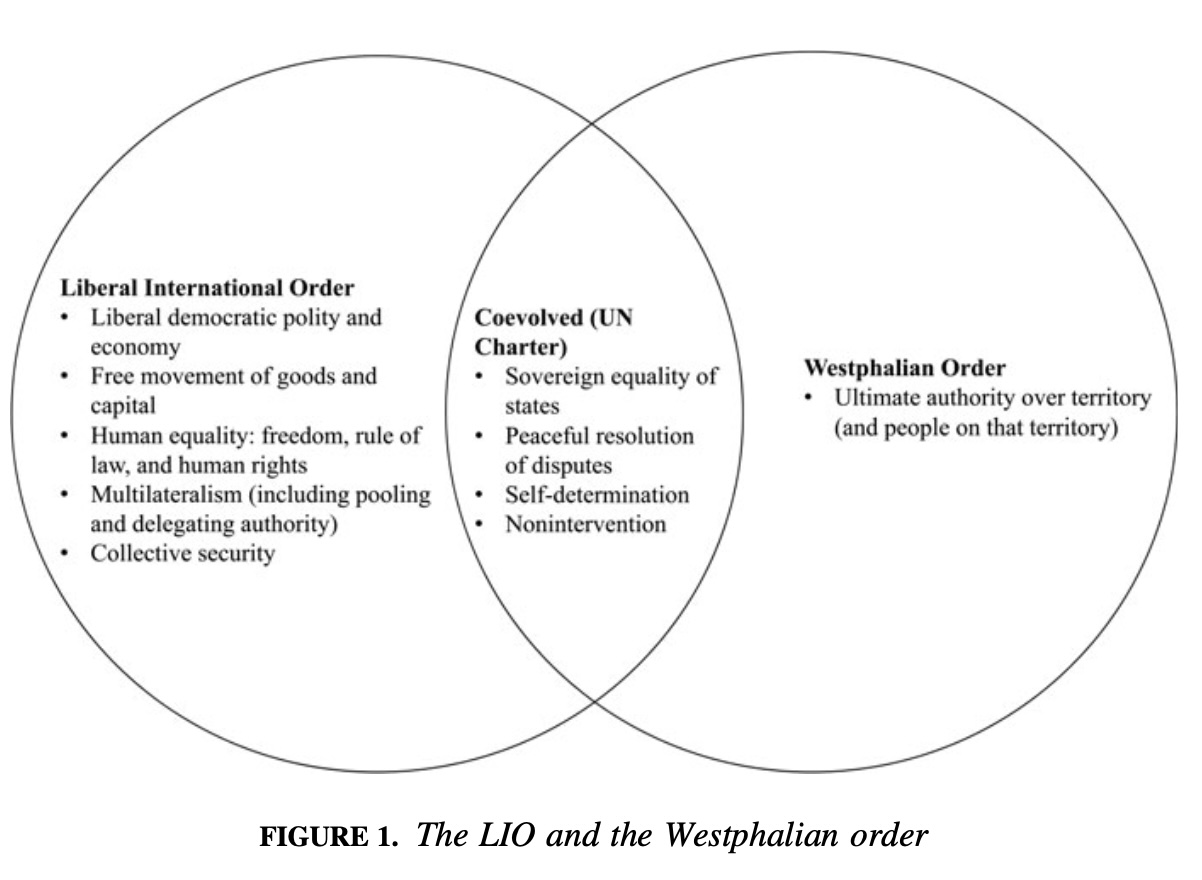
\includegraphics[width=1\textwidth]{images/challenges_to_liberal_order_LIO_vs_westphalian.jpg}
    \captionof{figure}{\label{fig:fig6_challenges_to_liberal_order_LIO_vs_westphalian.jpg}%\textit{\parencite[Fig.\(\backsim\)1]{cranmerWhatCanWe2017}}
    }
\end{center}

\subsection{Liberal: Political Liberalism}
At its philosophical core, liberalism rests on universal human equality, freedom, and individual and collective self-determination. Political liberalism therefore implies the rule of law, representative government, political participation, and protection of individual rights.

Institutions such as the International Criminal Court and doctrines such as the Responsibility to Protect illustrate how the LIO can authorize constraints on domestic sovereignty in the name of universal rights.

\subsection{Economic Liberalism and Embedded Liberalism}

A classical version favors market capitalism, free trade, international capital mobility, and equal treatment of foreign investment.

A second, historically important version is embedded liberalism. The postwar architects of the Bretton Woods system combined trade liberalization with domestic welfare states.

The distinction is important because economic liberalism does not automatically contradict Westphalian sovereignty.

The LIO broadly liberalized goods, services, and capital but never generally established free movement of labor outside the EU.

\subsection{Liberal Internationalism}

The institutional dimension of the LIO is based on principled multilateralism. Multilateralism means more than coordination among several states: it means coordination according to generalized rules that apply across cases rather than ad hoc bargaining based solely on particular interests. The GATT,WTO and UN Charter exemplify this logic. Liberal internationalism also includes peaceful dispute resolution, the ambition to provide global public goods, security communities such as NATO, and multilateral arms-control and nonproliferation regimes.

\textbf{Tensions with Westphalia:}
\begin{enumerate}
    \item Authority is delegated supranational bodies
    \item Majority voting
    \item Dispute-settlement mechanisms
    \item International courts.
\end{enumerate}

\subsection{Universalism and Selective Participation}

The LIO contains a paradox. Because liberalism begins from universal equality, the order is in principle open to all states. Yet states can join important parts of the LIO without being liberal democracies.

The LIO is therefore best understood as an evolving order whose components vary in reach rather than as a single uniform system imposed everywhere by the United States.

\subsection{Challenges from Within the Liberal Core}

The most striking contemporary threats come not only from geopolitical rivals but also from the internal workings of liberalism itself. The authors identify several mechanisms through which the LIO generates opposition within its own core members.

\begin{enumerate}
    \item Economic liberalism creates winners and losers. Trade openness, technological change, global production chains, and the financial crisis of 2008--2010 have produced geographically concentrated losses and contributed to rising inequality.
    \item Political openness can be used against liberalism. Freedom of expression and the open architecture of the internet allow misinformation, foreign influence, and strategies of "truth subversion" to circulate widely. 
    \item Free-trade policies and supranational governance were sometimes insulated from popular pressure in order to prevent protectionism and secure long-term cooperation. Over time, however, this technocratic insulation excluded some constituencies and created resentment. International institutions appeared less responsive to citizens.
    \item liberal universalism collides with national identity. Who belongs to the national community? Migration is a problem
\end{enumerate}

\subsection{Nationalist Populism and Political Realignment}

These pressures converge in movements combining nationalism, populism, and authoritarianism. Nationalism prioritizes the interests and identity of a particular state; populism pits a supposedly homogeneous "people" against elites and pluralist institutions; authoritarianism rejects liberal constraints such as independent courts, a free press, and fair electoral competition.

\subsection{External Challengers}

\begin{itemize}
    \item Climate change
    \item Distributional conflicts due to Climate change
    \item China: Its extraordinary economic growth was enabled by participation in the open international economy, yet China remains authoritarian and strongly defends sovereignty and noninterference.
\end{itemize}

\subsection{The Erosion of Multilateral Institutions}

Internal and external challenges converge most directly in attacks on multilateralism. Multilateral institutions have experienced crises before, including the collapse of the Bretton Woods monetary system and the US decision to invade Iraq without broad UN support. What appears different in the contemporary period is the breadth of skepticism and the willingness of major states to weaken institutions without a clear systemic necessity.

\begin{enumerate}
    \item WTO crisis: Even before the recent crisis it struggled to negotiate large new trade agreements. The United States combined protectionist tariffs with a strategy of blocking appointments to the WTO Appellate Body, impairing enforcement.
    \item Refugee crisis: The refugee regime illustrates a broader erosion of multilateral commitments. The principle of nonrefoulement and the 1951 Refugee Convention created legal obligations toward asylum seekers, yet receiving states have increasingly adopted restrictive or deterrent policies.
\end{enumerate}

\subsection{Sources of Resilience}

\begin{enumerate}
    \item the order has produced substantial benefits: reduced conflict among core members, economic growth, lower global poverty, and extensive international cooperation.
    \item LIO has generated vested interests: Firms have built global investments and supply chains that depend on open trade and predictable international rules. The same interdependence that creates vulnerability can also reinforce support for openness.
    \item the LIO institutions can outlast the circumstances that produced them and act as shock absorbers during crises.
    \item \textbf{Legitimacy}: After decades of operation, many rules of multilateral cooperation have acquired a sense of normality and rightfulness. Practices that once required active justification can become taken for granted as normal components of international life.
    
    \textbf{Accumulated normative capital}
    
    \textbf{Political baseline}
\end{enumerate}

\subsection{Four Analytic Blind Spots in IR Scholarship}

\begin{enumerate}
    \item \textbf{Exclusion}, stigma, and the threat of losing membership help enforce order. Exclusion is not merely a defect at the margins of the LIO.
    \item \textbf{Orders Are Not Neutral:} distributional consequences and the fact that rules are written by particular actors for particular purposes. Cooperation can be Pareto-improving while still distributing gains unequally.
    \item \textbf{Institutions Depend on Social Foundations:} Institutions survive because social groups invest political resources in creating and defending them. Institutional insulation may sometimes be necessary to protect long-term cooperation from short-term pressures.
    \item \textbf{Domestic Politics Can Challenge the Order Itself:} IR scholarship  paid little attention to the possibility that parties, protest movements, territorial cleavages, and mass political realignments inside core states could attack the international order itself.
\end{enumerate}

\subsection{USA and the Future of LIO}
Question about American leadership.

\begin{itemize}
    \item The LIO could survive because existing institutions and old and new stakeholders defend it.
    \item more traditional Westphalian order centered on sovereignty and noninterference.
    \item It could be transformed into a hybrid order that preserves economic openness and principled multilateralism while altering commitments to democracy, human rights, and international legal authority.
\end{itemize}

\newpage
\part{Text as Data}
%\textbf{Session 3, February 23: The strategic perspective}

\begin{itemize}
    \item [***] \textcite[Introduction]{cranmerWhatCanWe2017}
    \item \textcite[Chapter 1]{cranmerWhatCanWe2017}
    \item \textcite[Chapter 2]{cranmerWhatCanWe2017}
\end{itemize}

% \begin{center}
%     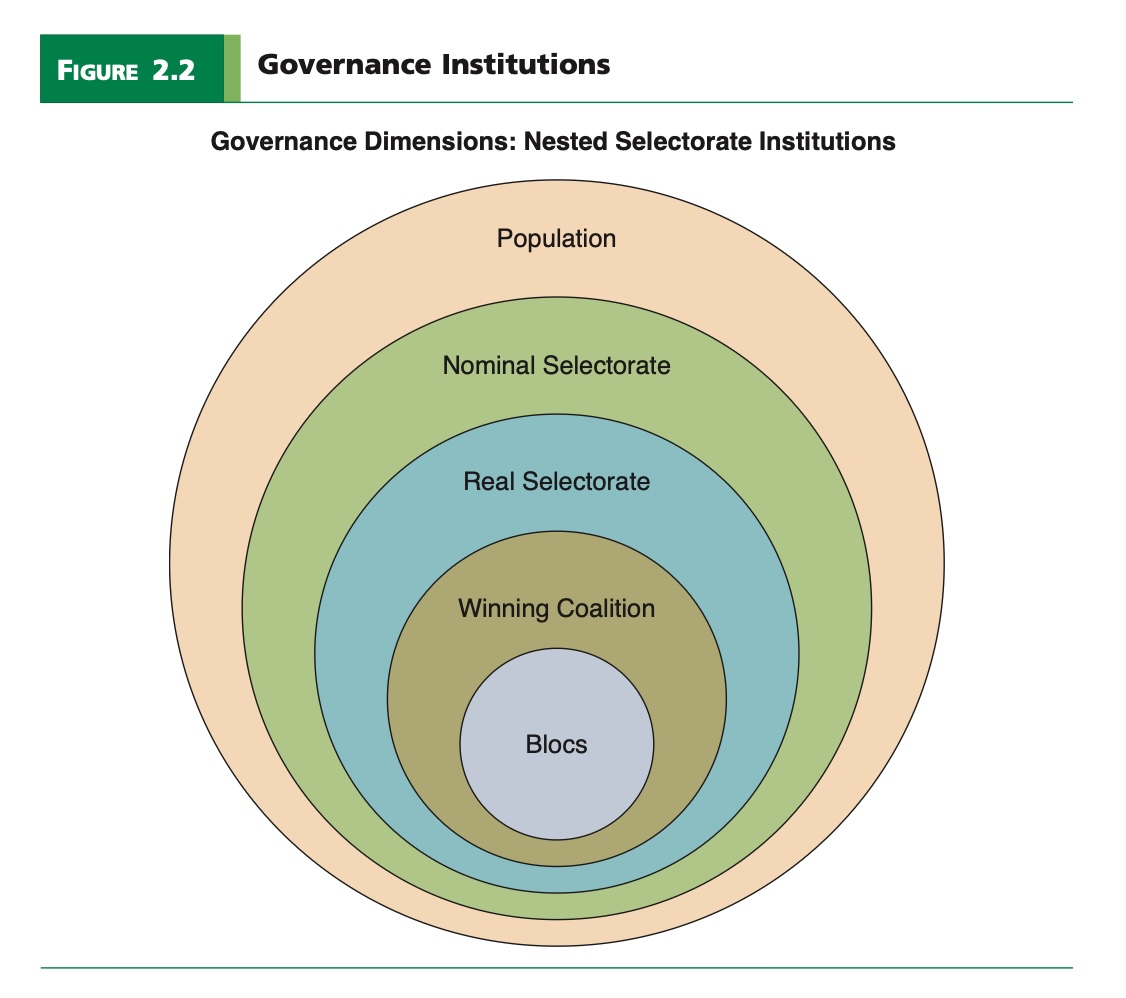
\includegraphics[width=0.7\textwidth]{images/nested_selectorate_institutions.jpg}
%     \captionof{figure}{\label{fig:fig3_nested_selectorate_institutions}%\textit{\parencite[Fig.\(\backsim\)1]{cranmerWhatCanWe2017}}
%     }
% \end{center}

\section{Semantic Role Labelling}


\subsection{SELECTORATE THEORY}
The selectorate theory represents one version of the strategic perspective.

In selectorate theory, leaders build a coalition of supporters among the selectorate. The selectorate (S) consists of those who have at least a nominal say in choosing leaders and are eligible to become members of a winning coalition. The winning coalition (W) is the subset of the selectorate without whose support an incumbent cannot be sustained in office.

\textbf{Leaders attempt to retain the loyalty of their supporters by giving them more benefits than any domestic political opponent can credibly promise to deliver.}
Rewards come in two varieties:


\begin{enumerate}
    \item [(1)] private goods:
    \item [] Private goods are rewards that benefit only those who get them—that is, members of the leader’s essential coalition of supporters.
    \item [] Examples might include privileged access to government contracts, exploitation of a black market, or protection against prosecution.
    \item [(2)] public goods.
    \item [] Public goods are government policies and programs that all people benefit from whether they are in the leader’s inner circle or not.
    \item [] Examples of public goods include national defense, free speech and free assembly, public parks, equal protection under the law, and free access to education.
\end{enumerate}

The selectorate theory's five rules of governance are as follows:

\begin{enumerate}
    \item Depend on as few key people to keep you in power as possible.
    
    \item Draw that small group of essential coalition members from as large a pool of people as possible.
    
    \item Tax people as much as possible, subject to the constraints that they continue to work and pay taxes rather than take siestas, and that they are not made so miserable that they decide it is worthwhile to risk revolting rather than continue to live with the existing political system.
    
    \item Reward your essential backers just enough so they stick with you rather than shopping around for a new leader who might do more for them.
    
    \item Don't spend resources on benefiting the general population when those resources are needed to keep the loyalty of the members of your essential coalition.
\end{enumerate}

\begin{center}
    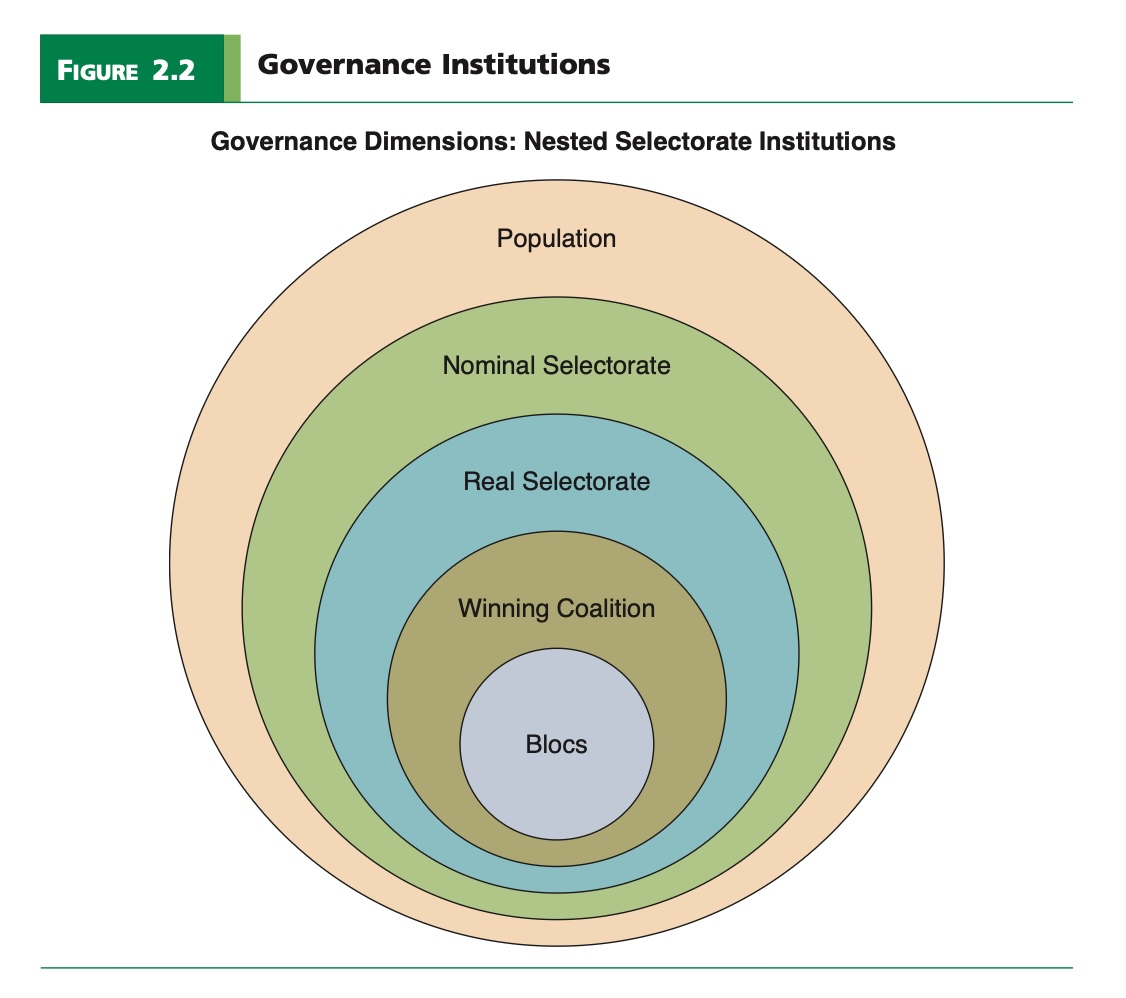
\includegraphics[width=0.7\textwidth]{images/nested_selectorate_institutions.jpg}
    \captionof{figure}{\label{fig:fig3_nested_selectorate_institutions}%\textit{\parencite[Fig.\(\backsim\)1]{cranmerWhatCanWe2017}}
    }
\end{center}

When domestic institutions constrain a leader to require a broad base of support private rewards are an inefficient way to retain power (de Tocqueville 2000; Lake and Baum 2001; Bueno de Mesquita et al. 2003; Bueno de Mesquita and Smith 2011). Democratic leaders would have to spread these rewards across so many people that each would receive too little for the benefits to influence their loyalty to the incumbent.

When political institutions compel a leader to depend on many supporters so that a bundle of public goods is the reward for retaining the incumbent, \textbf{the institutions of governance induce weak loyalty to the incumbent}.




%------- Bibliography -------
\newpage
\subsection*{\Large Bibliography}
\printbibliography[type=book, title={\large Books}]
\printbibliography[type=article, title={\large Articles}]


%------- Additional Material -------
% \newpage
% \begin{refsection}
%     \nocite{*}
%     \printbibliography[title={\Large Additional Material}, notcategory=cited]
% \end{refsection}

\end{document}
